%\documentclass[tikz,convert={outfile=\s1.svg}]{standalone}
\documentclass[tikz]{standalone}
\usepackage{amsthm}
\usepackage[landscape]{geometry}
\usepackage{multicol}
\usepackage{tikz}
\usepackage{pgfplots}
\usepackage{xcolor}
\usepackage{amsmath}
\usepackage[T1]{fontenc}
\usepackage{utopia}
\usepackage{changepage}
\usepackage{amssymb}
\usepackage{fancyhdr}
\usepackage[many]{tcolorbox}
\usepackage{moresize}
\usepackage{fullpage}
%\usepackage{mathpazo}
\usepackage{tikz-3dplot}
\usepackage{cancel}
\tdplotsetmaincoords{70}{165}
\pgfplotsset{compat=1.18}
\usepackage{enumitem}
\usepackage{tabularray}
\usepackage{mathtools}
\usepackage{pgfmath}

\UseTblrLibrary{diagbox}

\usetikzlibrary{
    shadings, calc, patterns, angles, quotes, arrows.meta, 
    decorations.pathmorphing, decorations.pathreplacing, 
    fadings, 3d, perspective, backgrounds, intersections, 
    decorations.markings, bending, positioning, 							spy,shapes.geometric,shadows,shapes.symbols, fadings, matrix, fit
}

\usepgfplotslibrary{
    groupplots, external, colormaps, patchplots, fillbetween
}


% Reds (r)
\definecolor{r1}{RGB}{255, 191, 191}    % Light coral
\definecolor{r2}{RGB}{255, 191, 223}    % Light pink
\definecolor{r3}{RGB}{255, 207, 207}    % Light rose

% Blues (b)
\definecolor{b1}{RGB}{191, 223, 255}    % Light blue
\definecolor{b2}{RGB}{191, 239, 255}    % Light sky
\definecolor{b3}{RGB}{191, 255, 255}    % Light cyan

% Greens (g)
\definecolor{g1}{RGB}{191, 255, 191}    % Light green
\definecolor{g2}{RGB}{191, 255, 223}    % Light mint
\definecolor{g3}{RGB}{207, 255, 207}    % Light sage

% Oranges (o)
\definecolor{o1}{RGB}{255, 223, 191}    % Light peach
\definecolor{o2}{RGB}{255, 239, 191}    % Light cream
\definecolor{o3}{RGB}{255, 231, 191}    % Light buff

% Violets (v)
\definecolor{v1}{RGB}{223, 191, 255}    % Light purple
\definecolor{v2}{RGB}{239, 191, 255}    % Light lilac
\definecolor{v3}{RGB}{231, 191, 255}    % Light lavender

% Yellows (y)
\definecolor{y1}{RGB}{255, 255, 191}    % Light yellow
\definecolor{y2}{RGB}{255, 247, 191}    % Light cream yellow
\definecolor{y3}{RGB}{255, 239, 191}    % Light warm cream

\definecolor{w}{HTML}{eeeeee}
\definecolor{g}{HTML}{444444}
\definecolor{b}{HTML}{222222}
\definecolor{lightgrey}{HTML}{cccccc}
\definecolor{firebrick}{RGB}{178, 34, 34}
\definecolor{myg}{RGB}{3, 252, 177}
\definecolor{mteal}{RGB}{73, 168, 143}


\color{w}
\begin{document}
\ssmall
%\pagecolor{b}
\nopagecolor
\fontfamily{put}

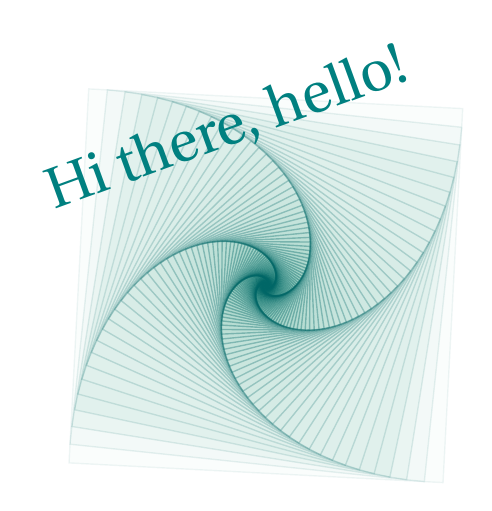
\begin{tikzpicture}[scale=1]
	\def\l{5}
	\def\n{120}
%	\pgfmathsetmacro{\t}{divide(1, \n)}
	\def\t{0.05}
	
	\coordinate (A0) at (0, 0);
	\coordinate (D0) at ($(A0) + (\l, 0)$);
	\coordinate (C0) at ($(A0) + (\l, \l)$);
	\coordinate (B0) at ($(A0) + (0, \l)$);	
	
%	\draw[draw=teal] (A0) -- (B0) -- (C0) -- (D0) -- cycle;
	
	\foreach \i in {1, ..., \n}{
%		\pgfmathtruncatemacro{\j}{\pgfmathsubtract(\i, 1)}
		\pgfmathtruncatemacro{\j}{subtract(\i, 1)}
		\pgfmathsetmacro{\of}{ifthenelse(\i < 5, sqrt(divide(\i, multiply(\n, 10))), divide(\i, multiply(\n, 13))}
		\pgfmathsetmacro{\od}{sqrt(divide(\i, multiply(\n, 2)))}
		\pgfmathsetmacro{\nt}{ifthenelse(\i < 90, \t, multiply(\t, 4))}
		\coordinate (A\i) at ($(A\j)!\nt!(B\j)$);
		\coordinate (B\i) at ($(B\j)!\nt!(C\j)$);
		\coordinate (C\i) at ($(C\j)!\nt!(D\j)$);
		\coordinate (D\i) at ($(D\j)!\nt!(A\j)$);
				
		\filldraw[line width=0.5, draw=teal!80!black, fill=mteal,fill opacity=\of, draw opacity=\od ] (A\i) -- (B\i) -- (C\i) -- (D\i) -- cycle;
	}
	
%	\node[text=teal, rotate=20] at ($(0, \l) + (2, -0.5)$) {{\fontfamily{pcr}\selectfont \huge Hi there, hello!}};
	\node[text=teal, rotate=20] at ($(0, \l) + (2, -0.5)$) {\huge Hi there, hello!};
\end{tikzpicture}

\end{document}